% Drawing 154/06-17 -- folder 154, batch 06, archive page 119 (PDF page 120).
% Transcription: à gauche, des dessins en couleur et au crayon : une droite vert clair traversée par deux croisements de droites rouges, entourée d'un contour vert foncé fléché dont les arcs sont numérotés $1$ à $4$ ; une courbe qui passe d'une hauteur à l'autre à travers un croisement, les régions hachurées ; un croisement enjambé par des courbes, régions numérotées $1$ à $7$ ; un disque et un ruban en huit au crayon ; en bas au milieu, un croisement de droites rouges avec deux courbes vert foncé et vert clair
% Kind: line with two crossings and a numbered contour; curve passing through a crossing; crossing straddled by curves; crossing with two green curves. Method 2 (schematic redraw from the facsimile). Status: partial.
% Notes: Left, colour and pencil drawings, read from the page view: a light green line crossed by two crossings of red lines, surrounded by an arrowed dark green contour whose arcs are numbered 1 to 4 (numbers placed approximately; a thick black segment on the line between the crossings); a curve going from one height to the other through a crossing, the regions hatched (one hatched region drawn); a crossing straddled by curves, regions numbered 1 to 7 (only some numbers placed); a pencil disk and a figure-eight ribbon (the disk drawn, the ribbon left out); bottom middle, a crossing of red lines with two curves, dark green and light green. The large ink blots in the middle of the sheet are stains, not drawings.
% Coordinates: 1 unit = 1 mm = 1/100 of the crop width (bbox in page fractions: [0.134, 0.114, 0.628, 0.473]).
% Redrawn by Claude (claude-opus-5-5), issue #73, 2026-11-07; not checked by a human; not compiled (no TeX in the session).
% Rights: reproduces part of the work -- behind RENDER_TRANSCRIPTS, never published by itself.
\documentclass[tikz,border=3pt]{standalone}
\usepackage{amsmath,amssymb}
\usetikzlibrary{patterns,arrows.meta}
\tikzset{Or/.style={orange!90!black}, Ye/.style={yellow!80!orange}, Lg/.style={green!60!black!70}, Dg/.style={green!45!black}, Br/.style={brown!80!black}, Rd/.style={red!85!black}, Bl/.style={blue!70!black}, Gy/.style={black!40}, pencil/.style={black!45}, struck/.style={black!35}, mark/.style={circle,draw,inner sep=1.3pt}, pt/.style={circle,fill,inner sep=0.9pt}, opt/.style={circle,draw,fill=white,inner sep=1.1pt}}
\begin{document}
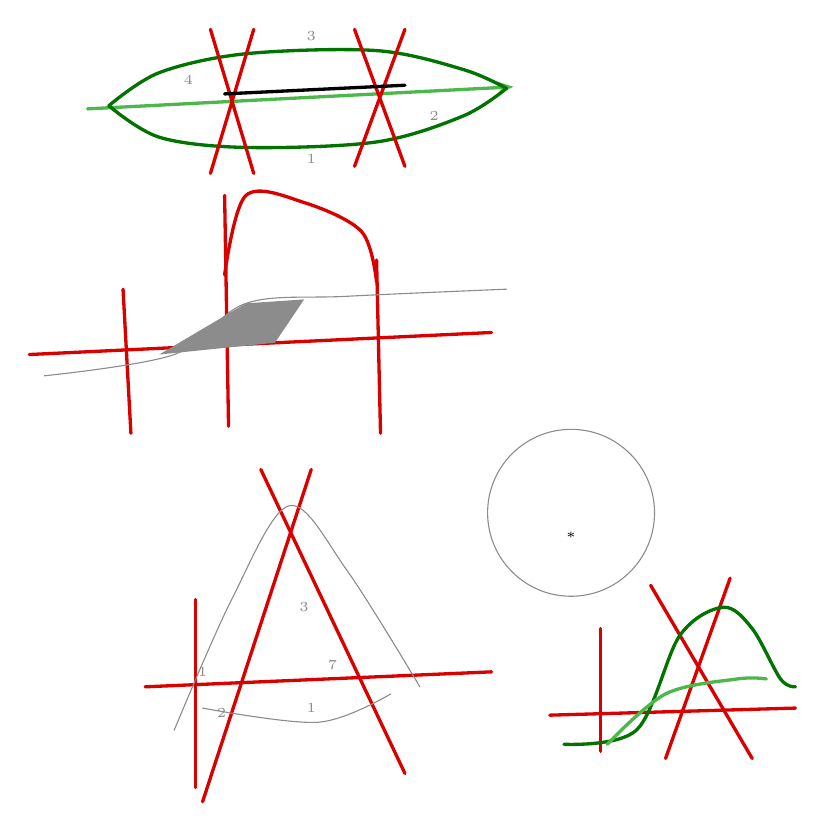
\begin{tikzpicture}[x=1mm,y=1mm,line cap=round,line join=round,font=\scriptsize]
\draw[Lg,very thick,-{Stealth[length=2mm]}] (8.3,-13.8) -- (62.4,-11);
\draw[Dg,very thick] plot[smooth, tension=0.55] coordinates {(11,-13.4) (17.4,-9.2) (28.4,-6.8) (45,-6.4) (56,-8.8) (61.5,-11.2)};
\draw[Dg,very thick] plot[smooth, tension=0.55] coordinates {(11,-13.4) (17.4,-17.4) (28.4,-18.7) (45,-18) (56,-14.7) (61.5,-11.2)};
\draw[Rd,very thick] (23.9,-3.7) -- (29.4,-22);
\draw[Rd,very thick] (29.4,-3.7) -- (23.9,-22);
\draw[Rd,very thick] (42.2,-3.7) -- (48.6,-21.1);
\draw[Rd,very thick] (48.6,-3.7) -- (42.2,-21.1);
\draw[very thick] (25.7,-11.9) -- (48.6,-10.8);
\node[inner sep=1pt,pencil] at (36.7,-4.6) {\tiny $3$};
\node[inner sep=1pt,pencil] at (36.7,-20.2) {\tiny $1$};
\node[inner sep=1pt,pencil] at (21.1,-10.1) {\tiny $4$};
\node[inner sep=1pt,pencil] at (52.3,-14.7) {\tiny $2$};
\draw[Rd,very thick] (0.9,-45) -- (59.6,-42.2);
\draw[Rd,very thick] (12.8,-36.7) -- (13.8,-55);
\draw[Rd,very thick] (25.7,-24.8) -- (26.2,-54.1);
\draw[Rd,very thick] (45,-33) -- (45.5,-55);
\draw[Rd,very thick] plot[smooth, tension=0.55] coordinates {(25.7,-34.9) (28.4,-24.8) (35.8,-25.7) (43.1,-29.4) (45,-35.8)};
\draw[pencil] plot[smooth, tension=0.55] coordinates {(2.8,-47.7) (19.3,-45) (28.4,-38.5) (41.3,-37.6) (61.5,-36.7)};
\fill[pattern=north east lines,pencil] (17.4,-45) -- (28.4,-38.5) -- (35.8,-38) -- (32.1,-43.5) -- cycle;
\draw[Rd,very thick] (15.6,-87.2) -- (59.6,-85.3);
\draw[Rd,very thick] (30.3,-59.6) -- (48.6,-98.2);
\draw[Rd,very thick] (36.7,-59.6) -- (22.9,-101.8);
\draw[Rd,very thick] (22,-76.1) -- (22,-100);
\draw[pencil] plot[smooth, tension=0.55] coordinates {(19.3,-92.7) (26.6,-76.1) (33.9,-64.2) (41.3,-72.5) (50.5,-87.2)};
\draw[pencil] plot[smooth, tension=0.55] coordinates {(22.9,-89.9) (37.6,-91.7) (46.8,-88.1)};
\node[inner sep=1pt,pencil] at (22.9,-85.3) {\tiny $1$};
\node[inner sep=1pt,pencil] at (25.3,-90.5) {\tiny $2$};
\node[inner sep=1pt,pencil] at (35.8,-77.1) {\tiny $3$};
\node[inner sep=1pt,pencil] at (36.7,-89.9) {\tiny $1$};
\node[inner sep=1pt,pencil] at (39.4,-84.4) {\tiny $7$};
\draw[pencil] (69.7,-65.1) circle[radius=10.6];
\node[inner sep=1pt] at (69.7,-67.9) {\tiny $*$};
\draw[Rd,very thick] (79.8,-74.3) -- (92.7,-96.3);
\draw[Rd,very thick] (89.9,-73.4) -- (81.7,-96.3);
\draw[Rd,very thick] (67,-90.8) -- (98.2,-89.9);
\draw[Rd,very thick] (73.4,-79.8) -- (73.4,-95.4);
\draw[Dg,very thick] plot[smooth, tension=0.55] coordinates {(68.8,-94.5) (78,-92.7) (83.5,-80.7) (89,-77.1) (92.7,-79.8) (96.3,-86.2) (98.2,-87.2)};
\draw[Lg,very thick] plot[smooth, tension=0.55] coordinates {(74.3,-94.5) (81.7,-88.1) (90.8,-86.2) (94.5,-86.2)};
\end{tikzpicture}
\end{document}
